%% ****** Start of file apstemplate.tex ****** %
%%
%%
%%   This file is part of the APS files in the REVTeX 4.2 distribution.
%%   Version 4.2a of REVTeX, January, 2015
%%
%%
%%   Copyright (c) 2015 The American Physical Society.
%%
%%   See the REVTeX 4 README file for restrictions and more information.
%%
%
% This is a template for producing manuscripts for use with REVTEX 4.2
% Copy this file to another name and then work on that file.
% That way, you always have this original template file to use.
%
% Group addresses by affiliation; use superscriptaddress for long
% author lists, or if there are many overlapping affiliations.
% For Phys. Rev. appearance, change preprint to twocolumn.
% Choose pra, prb, prc, prd, pre, prl, prstab, prstper, or rmp for journal
%  Add 'draft' option to mark overfull boxes with black boxes
%  Add 'showkeys' option to make keywords appear
% \documentclass[aps,prl,preprint,groupedaddress]{revtex4-2}
% \documentclass[aps,prl,preprint,superscriptaddress]{revtex4-2}
%\documentclass[aps,prl,reprint,groupedaddress]{revtex4-2}

\documentclass[%
 reprint,
superscriptaddress,
%groupedaddress,
%unsortedaddress,
%runinaddress,
%frontmatterverbose,
%preprint,
%preprintnumbers,
%nofootinbib,
%nobibnotes,
%bibnotes,
 amsmath,amssymb,
 aps,
%pra,
%prb,
%rmp,
%prstab,
%prstper,
floatfix,
]{revtex4-2}


\usepackage{graphicx}
\usepackage[version=4]{mhchem}

\newcommand{\cufegao}{CuFe$_{1-x}$Ga$_{x}$O$_{2}$ ($x$ = 0.035)}


% You should use BibTeX and apsrev.bst for references
% Choosing a journal automatically selects the correct APS
% BibTeX style file (bst file), so only uncomment the line
% below if necessary.
%\bibliographystyle{apsrev4-2}

\begin{document}

% Use the \preprint command to place your local institutional report
% number in the upper righthand corner of the title page in preprint mode.
% Multiple \preprint commands are allowed.
% Use the 'preprintnumbers' class option to override journal defaults
% to display numbers if necessary
%\preprint{}

%Title of paper
\title{Polarized neutron scattering in high magnetic fields using a long pulsed magnet}

% repeat the \author .. \affiliation  etc. as needed
% \email, \thanks, \homepage, \altaffiliation all apply to the current
% author. Explanatory text should go in the []'s, actual e-mail
% address or url should go in the {}'s for \email and \homepage.
% Please use the appropriate macro foreach each type of information

% \affiliation command applies to all authors since the last
% \affiliation command. The \affiliation command should follow the
% other information
% \affiliation can be followed by \email, \homepage, \thanks as well.
\author{Shingo~Takahashi}
\affiliation{Institute for Solid State Physics, The University of Tokyo, Kashiwa, Chiba 277-8581, Japan}
\affiliation{J-PARC Center, Japan Atomic Energy Agency, Tokai, Ibaraki 319-1195, Japan}

\author{Yuta~Osawa}
\affiliation{Institute for Solid State Physics, The University of Tokyo, Kashiwa, Chiba 277-8581, Japan}

\author{Yasuhiro~Inamura}
\affiliation{J-PARC Center, Japan Atomic Energy Agency, Tokai, Ibaraki 319-1195, Japan}

\author{Kazuki~Ohishi}
\affiliation{J-PARC Center, Japan Atomic Energy Agency, Tokai, Ibaraki 319-1195, Japan}

\author{Yukihiko~Kawamura}
\affiliation{J-PARC Center, Japan Atomic Energy Agency, Tokai, Ibaraki 319-1195, Japan}

\author{Masaki~Gen}
\affiliation{Institute for Solid State Physics, The University of Tokyo, Kashiwa, Chiba 277-8581, Japan}

\author{Hiroaki~Fujikawa}
\affiliation{Institute for Solid State Physics, The University of Tokyo, Kashiwa, Chiba 277-8581, Japan}

\author{Sharma~Vikash}
\affiliation{Institute for Solid State Physics, The University of Tokyo, Kashiwa, Chiba 277-8581, Japan}

\author{Toshiaki~Morikawa}
\affiliation{Institute for Solid State Physics, The University of Tokyo, Kashiwa, Chiba 277-8581, Japan}

\author{Masao~Watanabe}
\affiliation{J-PARC Center, Japan Atomic Energy Agency, Tokai, Ibaraki 319-1195, Japan}

\author{Taro~Nakajima}
\affiliation{Institute for Solid State Physics, The University of Tokyo, Kashiwa, Chiba 277-8581, Japan}
\affiliation{Institute of Materials Structure Science, High Energy Accelerator Research Organization, Tsukuba, Ibaraki 305-0801, Japan}
\affiliation{RIKEN Center for Emergent Matter Science, Wako, Saitama 351-0198, Japan}

\author{Yoshimitsu~Kohama}
\affiliation{Institute for Solid State Physics, The University of Tokyo, Kashiwa, Chiba 277-8581, Japan}

%Collaboration name if desired (requires use of superscriptaddress
%option in \documentclass). \noaffiliation is required (may also be
%used with the \author command).
%\collaboration can be followed by \email, \homepage, \thanks as well.
%\collaboration{}
%\noaffiliation

\date{\today}

\begin{abstract}
% insert abstract here
\end{abstract}

% insert suggested keywords - APS authors don't need to do this
%\keywords{}

%\maketitle must follow title, authors, abstract, and keywords
\maketitle

% body of paper here - Use proper section commands
% References should be done using the \cite, \ref, and \label commands
% Put \label in argument of \section for cross-referencing
%\section{\label{}}
\section{Introduction}

Magnetic fields are one of the most beneficial environments for material research because they can directly influence the electron orbital motion and spin in materials without direct contact.
A variety of emergent phenomena arising from magnetic ordering have attracted considerable attention in condensed matter physics.
To explore these field-induced magnetic phases, high-field magnet technologies have been extensively developed.

Meanwhile, neutron diffraction has played a central role in elucidating magnetic structures because it directly probes the spatial arrangement of magnetic moments in materials.
In particular, polarized neutron diffraction provides information on the orientation of magnetic moments by exploiting the spin-dependent scattering of neutrons.
% Neutron diffraction under high magnetic fields is a powerful technique for investigating field-induced phase transitions, as it directly probes changes in magnetic structures that cannot be fully determined from macroscopic measurements alone.
However, neutron diffraction experiments under high magnetic fields remain technically challenging.
Although superconducting magnets provide steady magnetic fields, their maximum fields are generally limited.
% Pulsed magnets can generate higher magnetic fields, but their short pulse durations often restrict the accessible neutron wavelength range and reciprocal space, particularly in time-of-flight (TOF) neutron diffraction experiments.

Recently, stroboscopic TOF neutron diffraction using a long pulsed magnet has been demonstrated at the Materials and Life Science Experimental Facility (MLF) of the Japan Proton Accelerator Research Complex (J-PARC) \cite{nakajima_stroboscopic_2024}.
By extending the magnetic-field pulse duration to more than 100 ms, this technique enables diffraction measurements over a broad neutron wavelength range under high magnetic fields.
Previous experiments successfully observed field-induced magnetic Bragg reflections and their magnetic-field dependence in triangular-lattice antiferromagnets up to 14 T.
% This long pulse duration and compact magnet design offer the potential for high-field polarized neutron diffraction.

In this study, we demonstrate stroboscopic TOF polarized neutron diffraction under long pulsed magnetic fields and apply this technique to CuFe$_{1-x}$Ga$_x$O$_2$ ($x=0.035$).
This compound exhibits a ferroelectric incommensurate magnetic phase with a proper-screw spin structure a propagation vector of $\mathbf{q}=(q,q,3/2)$ ($q \approx 0.203$) at zero magnetic field.
A field-induced phase transition occurs at approximately 10 T for a magnetic field applied along the $c$ axis.
Previous neutron diffraction measurements revealed changes in the magnetic Bragg reflection intensities across this transition \cite{nakajima_stroboscopic_2024}.
However, the magnetic structure of the high-field phase remains unclear, particularly the orientation of the magnetic moments.
We performed polarized neutron diffraction on this field-induced phase to investigate the magnetic structure of CuFe$_{1-x}$Ga$_x$O$_2$ ($x=0.035$) from the intensity ratio of non-spin-flip (NSF) to spin-flip (SF) scattering.
% By analyzing the non-spin-flip and spin-flip scattering intensities, we examine the orientation of the magnetic moments in the high-field phase.
% The experiments were performed at the TAIKAN diffractometer at J-PARC using a long pulsed magnet combined with neutron polarization analysis.
% We first evaluate the preservation of neutron polarization under pulsed magnetic fields and then measure the non-spin-flip and spin-flip scattering intensities of a magnetic Bragg reflection across the field-induced phase transition.
% By comparing these intensities, we investigate the orientation of the magnetic moments in the high-field phase and assess the applicability of polarized neutron diffraction to magnetic structure studies under high magnetic fields.
% In this study, we demonstrate stroboscopic time-of-flight polarized neutron diffraction under long pulsed magnetic fields to investigate the field-induced magnetic structure of \cufegao.


\section{Experimental Details}

% 全体のセットアップ
% 個々の装置

The polarized neutron diffraction experiments were performed at the small-angle and wide-angle neutron TOF diffractometer TAIKAN in MLF of J-PARC \cite{takata_design_2015}.
The experimental setup is shown in Fig.\ref{fig:setup}.
The sample position of TAIKAN is 14.35 m away from a neutron moderator.
A neutron wavelength range of TAIKAN is 0.7 to 7.7 \AA by the TOF method.
The detector of TAIKAN is composed of four detector banks of small-, middle-, high-angle, and backward detector banks.
Among these detector banks, the high-angle detector bank was used for the measurement of the magnetic reflection in high fields, and the small-angle detector bank was used for the evaluation of the total neutron polarization.
An incident neutron beam and scattered neutrons were polarized by a V-sharped Fe/Si supermirror.
Two guide magnetic which generate a magnetic field in vertical to maintain the neutron polarization were installed before and after the sample magnet.

The same single crystal of \cufegao\ used in Ref. \cite{nakajima_stroboscopic_2024} was employed in the present study.
The single crystal was oriented with the (HHL) plane as the scattering plane, allowing access to the magnetic reflection at $\boldsymbol{Q} = (q,q, 1.5)$ ($q=0.203$).
The sample was mounted in a closed-cycle refrigerator (CCR) and cooled to 4 K.



% The pulse interval was 10 minutes.

% Details of the sample preparation and characterization are described in Ref. \cite{}.

% 1. 磁石の基本仕様：装置を特定できる情報を簡潔に記載する。
% 2. 今回の実験条件：実際に使用した磁場強度、パルス幅、温度、磁場方向などを具体的に記載する。
% 3. 既報との差分：磁石や測定系に変更を加えた場合、その内容を明示する。
% 4. 先行研究の引用：磁石の設計・製作・性能評価については、既報を引用して重複した説明を避ける。
% 特に注意してほしいのは、装置の仕様（capability）と今回の実験で達成した条件（actual experimental conditions）を混同しないことです。
% 例えば、既報で15 Tまで繰り返し使用できることが示されていても、今回の実験で10 Tまでしか使用していなければ、実験条件としては10 Tと記載する必要があります。

Figure \ref{fig:tofdiagram} shows a temporal profile of the long pulsed magnetic field generated by a charging voltage of $V_c$ = 250 V.
The magnetic field reaches a maximum of approximately 12 T and then gradually decreases.
The vertical dashed line shows the time that 2.83 \AA neutrons which corresponds to the magnetic reflection of interest arrive at sample position of 14.35 m.
Since the critical field of \cufegao\ is $H_c \simeq 10 \mathrm{T}$, we dealt the neutron pulsed frame 2 and 3 corresponds to the phase transition data.
The pulsed interval was 10 minutes and repeated automatically.
More details of configuration of magnet is shown in \cite{nakajima_stroboscopic_2024}.

% As shown by the vertical dashed lines, neutrons of this wavelength from successive neutron pulses arrive at the sample at different times during the magnetic-field pulse.
% The critical field of \cufegao is $H_c \eqsim 10 \mathrm{T}$


\begin{figure}[h]
    \centering
    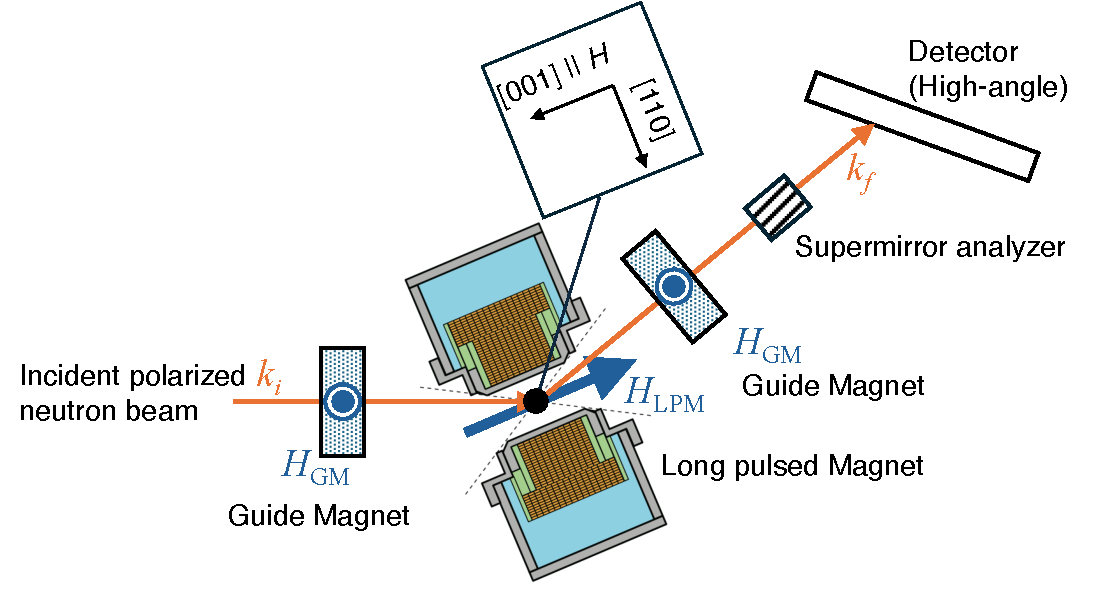
\includegraphics[width=\columnwidth]{figures/Setup_v1.pdf}
    \caption{
    Schematic illustration of the polarized neutron diffraction experiment.}
    \label{fig:setup}
\end{figure}



\begin{figure}[h]
    \centering
    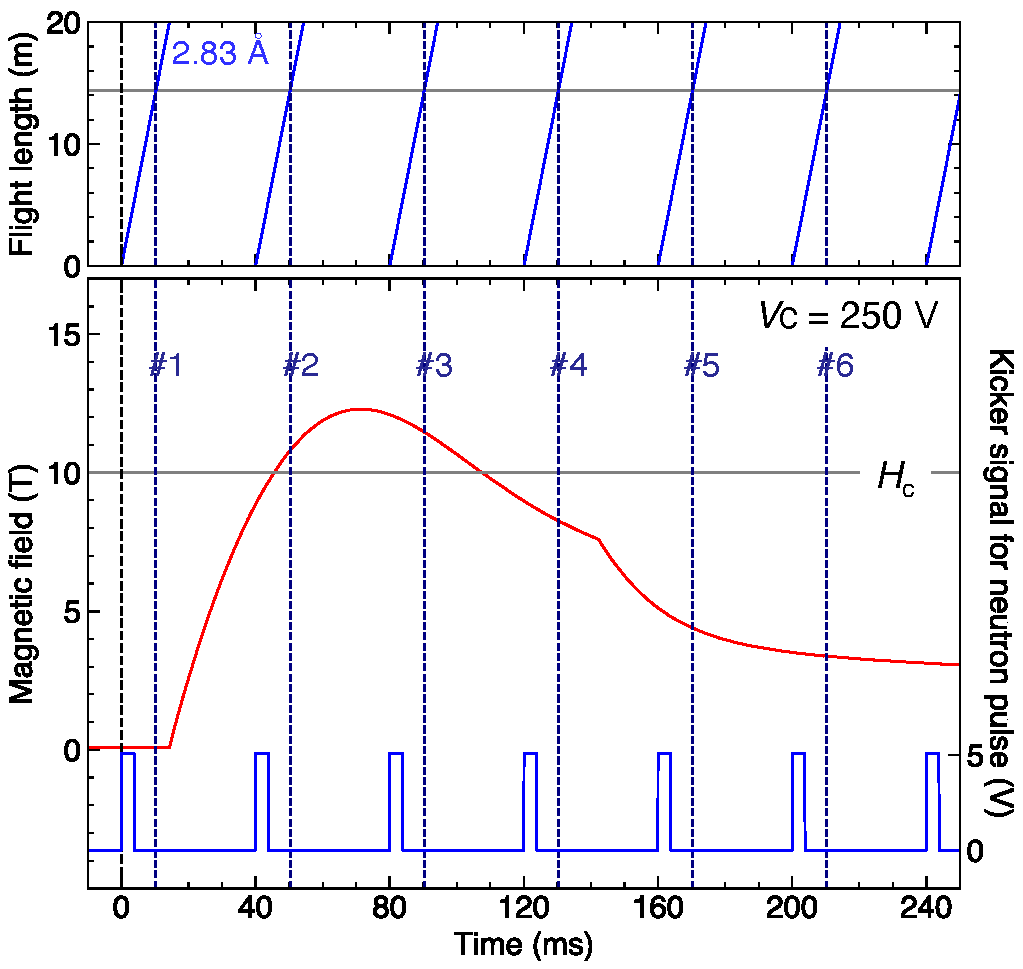
\includegraphics[width=\columnwidth]{figures/TOFdiagram_v1.pdf}
    \caption{
    Comparisons among the time-of-flight (TOF) diagram, the temporal profile of the long pulsed magnetic field generated with a charging voltage of 270 V, and the kicker signals for neutron pulse generation.
    The upper panel shows the flight paths of neutrons with a wavelength of 2.83 \AA, corresponding to the reflection of interest.
    The vertical dashed lines indicate the arrival times of 2.83 \AA \ neutrons from successive neutron pulses 1-6 at the sample position, which is 14.35 m away from the neutron source.
    The horizontal gray line indicates the critical field ($H_{\mathrm{c}}$).
    }
    \label{fig:tofdiagram}
\end{figure}

% \begin{figure}[h]
%     \centering
%     \includegraphics[width=\columnwidth]{figures/fig2.pdf}
%     \caption{one pulseの磁場波形と中性子パルスタイミングの模式図。}
%     \label{fig:one_pulse}
% \end{figure}


% \section{Results and Discussion}

% \subsection{Total neutron polarization}
% \begin{figure}[h]
%     \centering
%     \includegraphics[width=\columnwidth]{figures/fig3.pdf}
%     \caption{Total neutron polarization at each magnetic field.}
%     \label{fig:total_polarization}
% \end{figure}

\section{Results}
% 実験ではまず、全体の中性子偏極度評価を行い、その後、磁気反射の非対称度の測定が行われた。


\subsection{Total neutron polarization}
To evaluate the preservation of neutron polarization, the flipping asymmetry of the direct beam was measured using the small-angle detector bank.
The geometry for the magnetic reflection measurements differed from the direct-beam configuration primarily by a rotation of the outgoing neutron flight path around the sample position, with the relative arrangement of the guide magnet and supermirror analyzer maintained.
Therefore, the direct-beam measurement was used to assess the polarization transport efficiency relevant to the magnetic reflection measurements.

\begin{equation}
    P_0(\lambda) = \frac{I_\mathrm{off}(\lambda)-I_\mathrm{on}(\lambda)}{I_\mathrm{off}(\lambda)+I_\mathrm{on}(\lambda)},
\end{equation}
where $I_\mathrm{off}(\lambda)$ and $I_\mathrm{on}(\lambda)$ are the intensity when neutron spin flipper off and on, respectively.

The long pulsed magnet, downstream guide magnet and supermirror analyzer were placed transmission geometry.

Figure\ref{fig:polarization} shows the $P_0(\lambda)$ for applied magnetic field of long pulsed magnet was 1 mT (stable), 12 T, 4 T.
The stable data points of 1 mT were measured from applying DC power supply of 3 A to the long pulsed magnet.
The 12 T, 4 T were measured to apply pulse 30 times, and summing the data of frame \#2-\#3, and \#5-\#6, respectively.


The wavelength of interest magnetic reflection is $2.83 \AA$.
Total neutron polarization was almost same values between constant current and high field.
The $P_0$ of 0.6 at $2.83 \AA$ was used for the correction of magnetic reflection.


\begin{figure}
    \centering
    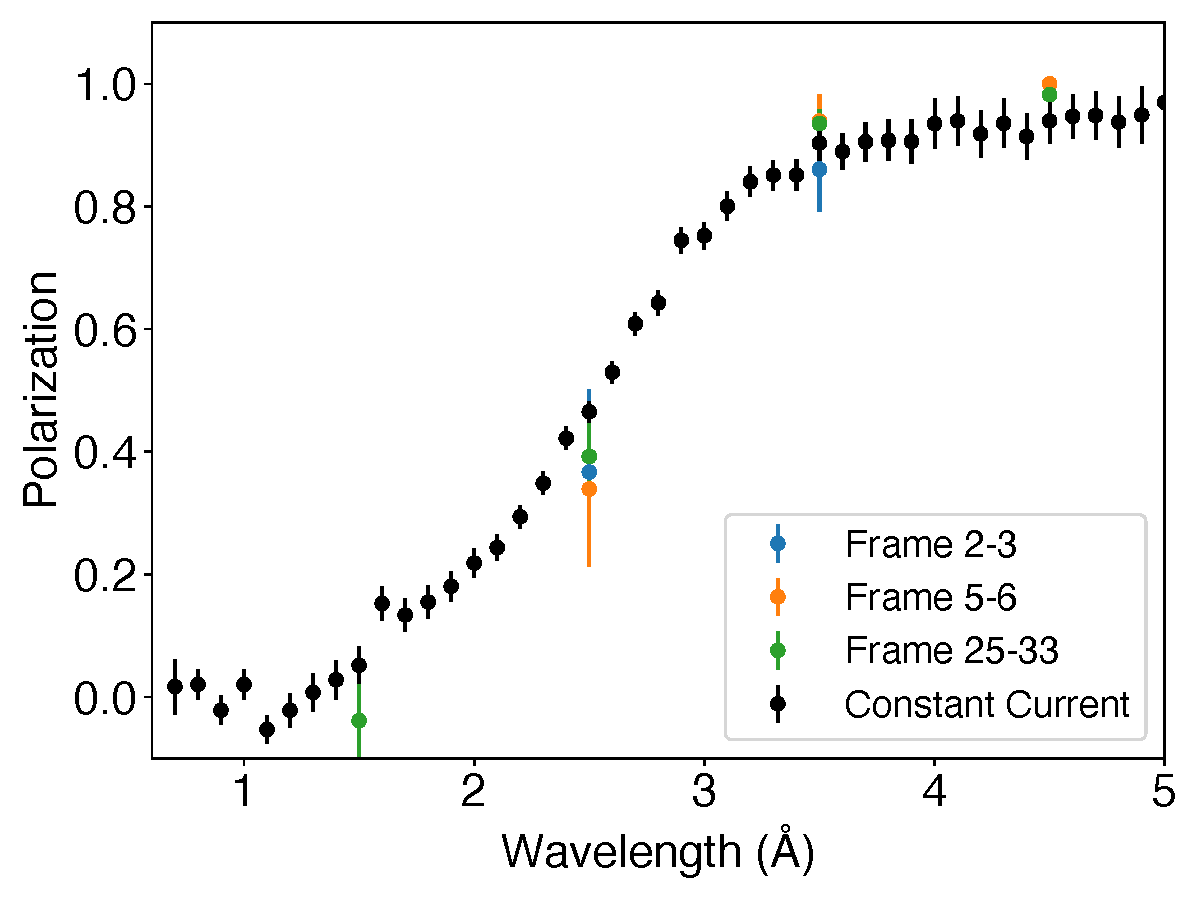
\includegraphics[width=\columnwidth]{figures/LPM_asymmetry_v1.pdf}
    \caption{
    Wavelength dependence of total neutron polarization at each magnetic fields.}
    \label{fig:total_pol}
\end{figure}


\subsection{Polarization analysis of a magnetic reflection}

We performed the stroboscopic TOF polarized neutron diffraction in long pulsed magnetic fields on \cufegao \ at 4K.
We repeated the application of the long pulsed magnetic field with the charging voltage of 250 V 62 times for $I_\mathrm{NSF}$ configuration and 61 times for $I_\mathrm{SF}$ configuration.
Figure \ref{fig:polarization_analysis} (a) shows the satellite reflection around (0, 1, -1), where frames 2 and 3, 5 and 6 summed together.
These correspond to magnetic fields of 12 tesla, 4 tesla, and 1 tesla, respectively.
The blue and red intensities correspond to NSF and SF scattering.
At 12 tesla, the relationship between these two intensities changes clearly compared with the lower-field data.
The lower-left figure shows the asymmetry calculated from these intensities and normalized to the beam polarization.
In the ground state, the magnetic structure has been already determined to be the helical structure, so the magnetic moments point in various directions.
In the present experimental setup, the NSF scattering corresponds to the c-axis component of the Fourier transformed magnetic moments.
The SF scattering corresponds to the in-plane component.
Both the spin components have nearly the same amplitudes in the ground state.
But by projecting all the spin components onto the plane perpendicular to the scattering vector, the contribution of the in-plane component to the magnetic scattering is slightly reduced.
As a result, the asymmetry was approximately 0.4.
This is consistent with the calculation shown by the dotted line.
At 12 tesla, however, the normalized asymmetry is almost 1, meaning that the magnetic scattering in the field-induced phase is almost entirely NSF scattering.
This indicates that the magnetic moments in the material have only c-axis components, parallel or antiparallel to the external field and to the neutron spin, and that they are arranged with the periodicity corresponding to this q vector.
Therefore, we conclude that the field-induced phase is a collinear ferrimagnetic structure with a 3-up, 2-down arrangement.
The critical fields of


Since the magnetic field was applied along the [001] direction, the non-spin flip intensity ($I_\mathrm{NSF}$) is caused by the Fourier transform magnetic moment with parallel to the neutron spin among the vertical component of scattering vector.
Other while, spin flip intensity is caused by the Fourier transform magnetic moment with vertical to the neutron spin among the vertical component of scattering vector.

\begin{figure}[h]
    \centering
    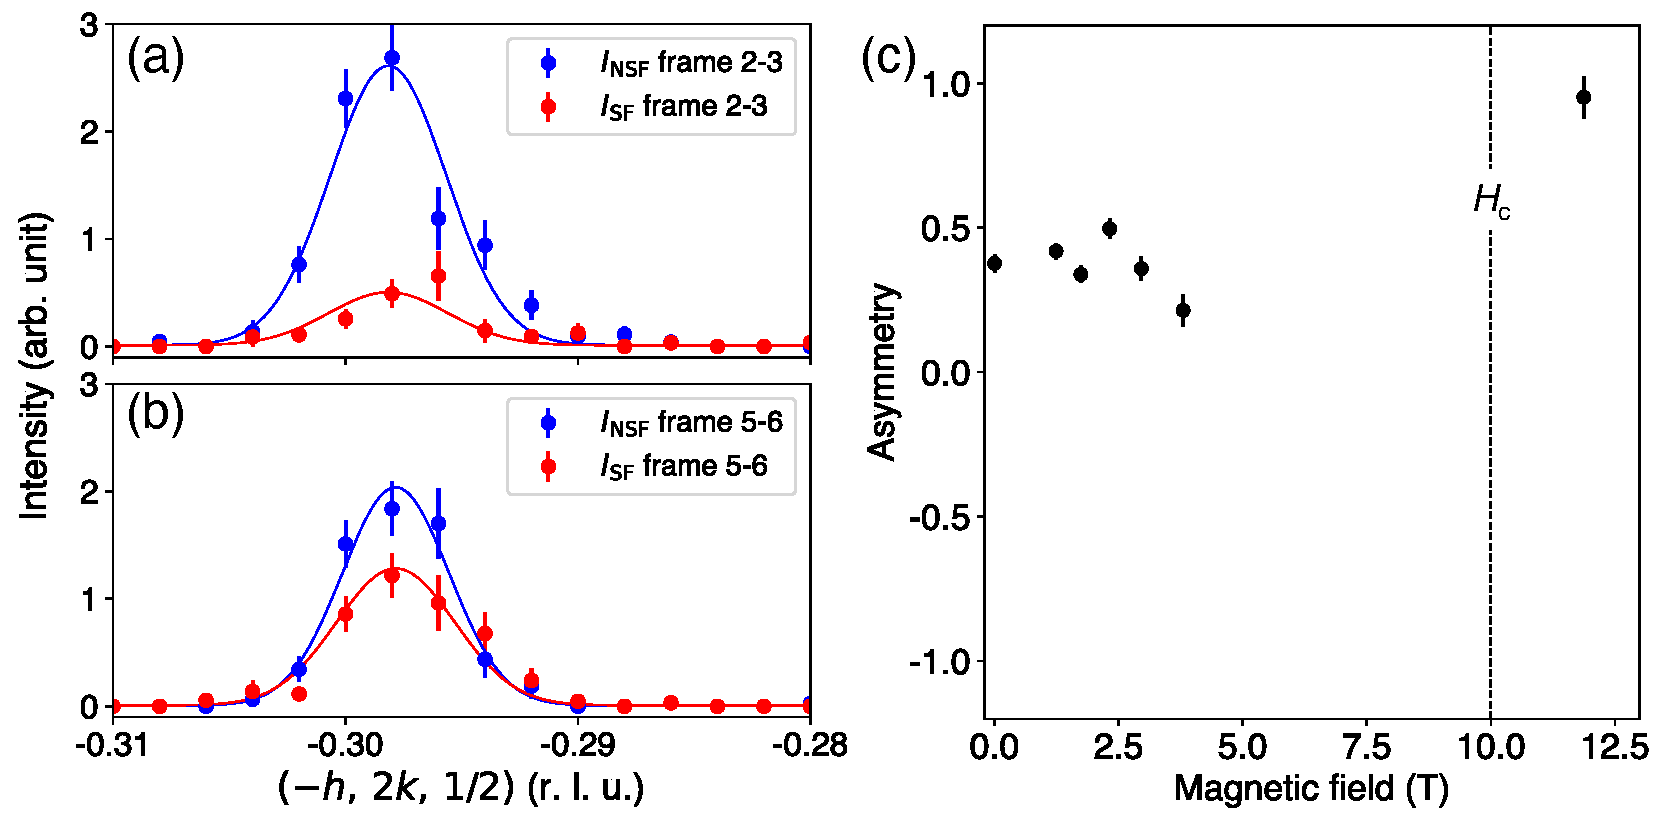
\includegraphics[width=\columnwidth]{figures/LPM_asy_v1.pdf}
    \caption{Polarization analysis of a magnetic reflection.}
    \label{fig:polarization_analysis}
\end{figure}




\section{Conclusion}
We conducted the stroboscopic TOF polarized neutron diffraction measurements with long pulsed magnetid fields at low temperatures.
We applied this technique to study the field-induced magnetic phase transitions of triangular lattice antiferromagnet \ce{CuFe_{1-x}Ga_{x}O_{2}} (x = 0.035) and successfully observed the field evolutions of the magnetic Bragg reflections up to 14 T.



\section{Acknowledgments}


\bibliography{ref}

\end{document}
%
% ****** End of file apstemplate.tex ******